% Generated 2020-10-22 16:25:26 +0530
\subsection{Observations} \label{sec:Observations}


\block{Observations} \glspl{organize} \block{Observation} elements.

\begin{figure}[ht]
  \centering
    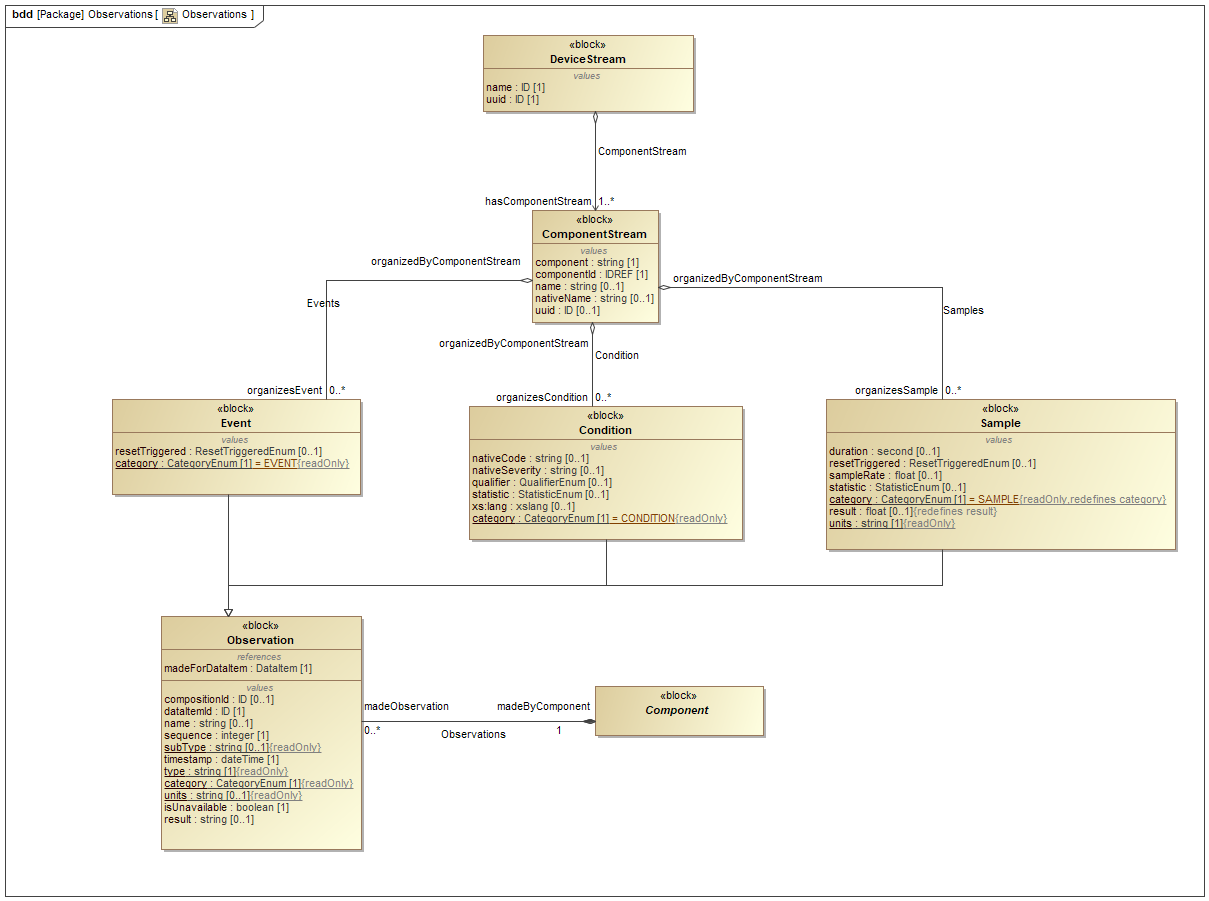
\includegraphics[width=1.0\textwidth]{figures/Observations.png}
  \caption{Observations Diagram}
  \label{fig:Observations}
\end{figure}

\FloatBarrier



\subsubsection{Observation}
\label{sec:Observation}



\block{Observation} provides telemetry data for a \block{DataItem} at a point in time.


\paragraph{Attributes of Observation}\mbox{}
\label{sec:Attributes of Observation}

\tbl{Attributes of Observation} lists the attributes of \texttt{Observation}.

\begin{table}[ht]
\centering 
  \caption{Attributes of Observation}
  \label{table:Attributes of Observation}
\tabulinesep=3pt
\begin{tabu} to 6in {|l|l|l|} \everyrow{\hline}
\hline
\rowfont\bfseries {Attribute} & {Type} & {Multiplicity} \\
\tabucline[1.5pt]{}
\property{compositionId}[Observation] & \texttt{ID} & 0..1 \\
\property{dataItemId}[Observation] & \texttt{ID} & 1 \\
\property{name}[Observation] & \texttt{string} & 0..1 \\
\property{sequence}[Observation] & \texttt{integer} & 1 \\
\property{subType}[Observation] & \texttt{string} & 0..1 \\
\property{timestamp}[Observation] & \texttt{dateTime} & 1 \\
\property{type}[Observation] & \texttt{string} & 1 \\
\property{category}[Observation] & \texttt{CategoryEnum} & 1 \\
\property{units}[Observation] & \texttt{string} & 0..1 \\
\property{result}[Observation] & \texttt{string} & 0..1 \\
\end{tabu}
\end{table}
\FloatBarrier


Descriptions for attributes of \block{Observation}:

\begin{itemize}

\item \property{compositionId}[Observation] : The identifier of the \block{Composition} element defined in the \block{MTConnectDevices} \gls{Response Document} associated with the data reported for the \block{Observation} element.

\item \property{dataItemId}[Observation] : The unique identifier for the \block{Observation} element.

\item \property{name}[Observation] : The name of the \block{Observation} element.

\item \property{sequence}[Observation] : A number representing the sequential position of an occurrence of an \gls{observation} in the data buffer of an \gls{Agent}.

\item \property{subType}[Observation] : The \property{subType} of the \block{Observation}.

\item \property{timestamp}[Observation] : The most accurate time available to a piece of equipment that represents the point in time that the data reported was measured.

\item \property{type}[Observation] : The \property{type} of the \block{Observation} element.

\item \property{category}[Observation] : The \property{category} of the \block{Observation} element.

\item \property{units}[Observation] : The \property{units} of the \block{Observation} element.

\item \property{result}[Observation] : The \gls{observation} of the \block{Observation} element.
\end{itemize}

\subsubsection{Condition}




\block{Condition} provides the information and data reported from a piece of equipment for those \block{DataItem} elements defined with a \property{category}[DataItem] attribute of \texttt{CONDITION} in the \block{MTConnectDevices} \gls{Response Document}.


\paragraph{Attributes of Condition}\mbox{}
\label{sec:Attributes of Condition}

\tbl{Attributes of Condition} lists the attributes of \texttt{Condition}.

\begin{table}[ht]
\centering 
  \caption{Attributes of Condition}
  \label{table:Attributes of Condition}
\tabulinesep=3pt
\begin{tabu} to 6in {|l|l|l|} \everyrow{\hline}
\hline
\rowfont\bfseries {Attribute} & {Type} & {Multiplicity} \\
\tabucline[1.5pt]{}
\property{nativeCode}[Condition] & \texttt{string} & 0..1 \\
\property{nativeSeverity}[Condition] & \texttt{string} & 0..1 \\
\property{qualifier}[Condition] & \texttt{QualifierEnum} & 0..1 \\
\property{statistic}[Condition] & \texttt{StatisticEnum} & 0..1 \\
\property{xs:lang}[Condition] & \texttt{xslang} & 0..1 \\
\property{category}[Condition] & \texttt{CONDITION} & 1 \\
\end{tabu}
\end{table}
\FloatBarrier


Descriptions for attributes of \block{Condition}:

\begin{itemize}

\item \property{nativeCode}[Condition] : The native code (usually an alpha-numeric value) generated by the controller of a piece of equipment providing a reference identifier for a \block{Condition}.

\item \property{nativeSeverity}[Condition] : If the piece of equipment designates a severity level to a fault, \property{nativeSeverity} reports that severity information to a client software application.

\item \property{qualifier}[Condition] : \property{qualifier} provides additional information regarding a \gls{Condition State} associated with the measured value of a process variable.

\tabulinesep = 5pt
\begin{longtabu} to \textwidth {
    |l|X|}
\caption{QualifierEnum Enumeration}
\label{enum:QualifierEnum} \\

\hline
Name & Description \\
\hline
\endfirsthead
\hline
\multicolumn{2}{|c|}{Continuation of Table \texttt{QualifierEnum} Enumeration} \\
\hline
Name & Description \\
\hline
\endhead
\texttt{HIGH} &  \\ \hline
\texttt{LOW} &  \\ \hline
\end{longtabu}


\item \property{statistic}[Condition] : \property{statistic} provides additional information describing the meaning of the \block{Condition} element.

\item \property{xs:lang}[Condition] : An optional attribute that specifies the language of the CDATA returned for the \block{Condition}. 

See \textit{IETF RFC 4646} (http://www.ietf.org/rfc/rfc4646.txt).
\end{itemize}

\subsubsection{Event}




\block{Event} provides the information and data reported from a piece of equipment for those \block{DataItem} elements defined with a \property{category}[DataItem] attribute of \texttt{EVENT} in the \block{MTConnectDevices} \gls{Response Document}.


\paragraph{Attributes of Event}\mbox{}
\label{sec:Attributes of Event}

\tbl{Attributes of Event} lists the attributes of \texttt{Event}.

\begin{table}[ht]
\centering 
  \caption{Attributes of Event}
  \label{table:Attributes of Event}
\tabulinesep=3pt
\begin{tabu} to 6in {|l|l|l|} \everyrow{\hline}
\hline
\rowfont\bfseries {Attribute} & {Type} & {Multiplicity} \\
\tabucline[1.5pt]{}
\property{resetTriggered}[Event] & \texttt{ResetTriggeredEnum} & 0..1 \\
\property{category}[Event] & \texttt{EVENT} & 1 \\
\end{tabu}
\end{table}
\FloatBarrier


Descriptions for attributes of \block{Event}:

\begin{itemize}

\item \property{resetTriggered}[Event] : For those \block{DataItem} elements that report data that may be periodically reset to an initial value, \property{resetTriggered} identifies when a reported value has been reset and what has caused that reset to occur.

\tabulinesep = 5pt
\begin{longtabu} to \textwidth {
    |l|X|}
\caption{ResetTriggeredEnum Enumeration}
\label{enum:ResetTriggeredEnum} \\

\hline
Name & Description \\
\hline
\endfirsthead
\hline
\multicolumn{2}{|c|}{Continuation of Table \texttt{ResetTriggeredEnum} Enumeration} \\
\hline
Name & Description \\
\hline
\endhead
\texttt{ACTION\textunderscore COMPLETE} & The value of the \block{Observation} that is measuring an action or operation was reset upon completion of that action or operation. \\ \hline
\texttt{ANNUAL} & The value of the \block{Observation} was reset at the end of a 12-month period. \\ \hline
\texttt{DAY} & The value of the \block{Observation} was reset at the end of a 24-hour period. \\ \hline
\texttt{MAINTENANCE} & The value of the \block{Observation} was reset upon completion of a maintenance event. \\ \hline
\texttt{MANUAL} & The value of the \block{Observation} was reset based on a physical reset action. \\ \hline
\texttt{MONTH} & The value of the \block{Observation} was reset at the end of a monthly period. \\ \hline
\texttt{POWER\textunderscore ON} & The value of the \block{Observation} was reset when power was applied to the piece of equipment after a planned or unplanned interruption of power has occurred. \\ \hline
\texttt{SHIFT} & The value of the \block{Observation} was reset at the end of a work shift. \\ \hline
\texttt{WEEK} & The value of the \block{Observation} was reset at the end of a 7-day period. \\ \hline
\end{longtabu}

\end{itemize}

\subsubsection{Sample}




\block{Sample} provides the information and data reported from a piece of equipment for those \block{DataItem} elements defined with a \property{category}[DataItem] attribute of \texttt{SAMPLE} in the \block{MTConnectDevices} \gls{Response Document}.


\paragraph{Attributes of Sample}\mbox{}
\label{sec:Attributes of Sample}

\tbl{Attributes of Sample} lists the attributes of \texttt{Sample}.

\begin{table}[ht]
\centering 
  \caption{Attributes of Sample}
  \label{table:Attributes of Sample}
\tabulinesep=3pt
\begin{tabu} to 6in {|l|l|l|} \everyrow{\hline}
\hline
\rowfont\bfseries {Attribute} & {Type} & {Multiplicity} \\
\tabucline[1.5pt]{}
\property{duration}[Sample] & \texttt{second} & 0..1 \\
\property{resetTriggered}[Sample] & \texttt{ResetTriggeredEnum} & 0..1 \\
\property{sampleRate}[Sample] & \texttt{float} & 0..1 \\
\property{statistic}[Sample] & \texttt{StatisticEnum} & 0..1 \\
\property{category}[Sample] & \texttt{SAMPLE} & 1 \\
\property{result}[Sample] & \texttt{float} & 0..1 \\
\property{units}[Sample] & \texttt{string} & 1 \\
\end{tabu}
\end{table}
\FloatBarrier


Descriptions for attributes of \block{Sample}:

\begin{itemize}

\item \property{duration}[Sample] : The time-period over which the data was collected.

\item \property{resetTriggered}[Sample] : For those \block{DataItem} elements that report data that may be periodically reset to an initial value, \property{resetTriggered} identifies when a reported value has been reset and what has caused that reset to occur.

\item \property{sampleRate}[Sample] : The rate at which successive samples of the value of a data item are recorded.

\property{sampleRate} is expressed in terms of samples per second.

\item \property{statistic}[Sample] : The type of statistical calculation defined by the \property{statistic} attribute of the \block{DataItem} element defined in the \block{MTConnectDevices} \gls{Response Document} that this element represents.
\end{itemize}

\paragraph{Elements of Sample}\mbox{}
\label{sec:Elements of Sample}

\tbl{Elements of Sample} lists the elements of \texttt{Sample}.

\begin{table}[ht]
\centering 
  \caption{Elements of Sample}
  \label{table:Elements of Sample}
\tabulinesep=3pt
\begin{tabu} to 6in {|l|l|l|} \everyrow{\hline}
\hline
\rowfont\bfseries {Element Name} & {Type} & {Multiplicity} \\
\tabucline[1.5pt]{}
\block{Samples} & \texttt{ComponentStream} & 1 \\
\end{tabu}
\end{table}
\FloatBarrier


Descriptions for elements of \block{Sample}:

\begin{itemize}
\item \block{Samples} : \block{Samples} \glspl{organize} the \texttt{SAMPLE} \property{category} type \block{DataItem} elements defined in the \block{MTConnectDevices} \gls{Response Document} that are reported in each \block{ComponentStream} element.
\end{itemize}
